% Slide: Algorithm 1: A Single Iteration
\begin{frame}{Algorithm 1: A Single Iteration}
  \begin{enumerate}
    \item \textbf{Update Spatial Random Effects \& Variance:} Update \(W\), \(\tau^2\), and \(\rho\) from their full conditionals based on the CAR prior.
    
    \item \textbf{Impute Censored Data:} For subjects $ij$, sample the latent log survival time as
      \[
      \tilde{y}_{ij} =
      \begin{cases}
        \operatorname{TruncNormal}\Bigl(\mu_{ij},\sigma^2;\log y_{ij}\Bigr), & \text{if } \delta_{ij}=0, \\[1ex]
        \log y_{ij}, & \text{if } \delta_{ij}=1.
      \end{cases}
      \]
    \item \textbf{Update BART:} With responses \(\tilde{y}_{ij} - W_i\) and covariates \((Z_{ij},\mathbf{X}_{ij})\), update the BART parameters \(\{\mathcal{T}_h,\mathcal{M}_h\}\) and the error variance \(\sigma^2\) via Bayesian backfitting.
    
  \end{enumerate}
\end{frame}% Options for packages loaded elsewhere
\PassOptionsToPackage{unicode}{hyperref}
\PassOptionsToPackage{hyphens}{url}
%
\documentclass[
  ignorenonframetext,
]{beamer}
\usepackage{pgfpages}
\setbeamertemplate{caption}[numbered]
\setbeamertemplate{caption label separator}{: }
\setbeamercolor{caption name}{fg=normal text.fg}
\beamertemplatenavigationsymbolsempty
% Prevent slide breaks in the middle of a paragraph
\widowpenalties 1 10000
\raggedbottom
\setbeamertemplate{part page}{
  \centering
  \begin{beamercolorbox}[sep=16pt,center]{part title}
    \usebeamerfont{part title}\insertpart\par
  \end{beamercolorbox}
}
\setbeamertemplate{section page}{
  \centering
  \begin{beamercolorbox}[sep=12pt,center]{part title}
    \usebeamerfont{section title}\insertsection\par
  \end{beamercolorbox}
}
\setbeamertemplate{subsection page}{
  \centering
  \begin{beamercolorbox}[sep=8pt,center]{part title}
    \usebeamerfont{subsection title}\insertsubsection\par
  \end{beamercolorbox}
}
\AtBeginPart{
  \frame{\partpage}
}
\AtBeginSection{
  \ifbibliography
  \else
    \frame{\sectionpage}
  \fi
}
\AtBeginSubsection{
  \frame{\subsectionpage}
}
\usepackage{amsmath,amssymb}
\usepackage{lmodern}
\usepackage{setspace}

\usepackage{iftex}
\ifPDFTeX
  \usepackage[T1]{fontenc}
  \usepackage[utf8]{inputenc}
  \usepackage{textcomp} % provide euro and other symbols
\else % if luatex or xetex
  \usepackage{unicode-math}
  \defaultfontfeatures{Scale=MatchLowercase}
  \defaultfontfeatures[\rmfamily]{Ligatures=TeX,Scale=1}
\fi
% Use upquote if available, for straight quotes in verbatim environments
\IfFileExists{upquote.sty}{\usepackage{upquote}}{}
\IfFileExists{microtype.sty}{% use microtype if available
  \usepackage[]{microtype}
  \UseMicrotypeSet[protrusion]{basicmath} % disable protrusion for tt fonts
}{}
\makeatletter
\@ifundefined{KOMAClassName}{% if non-KOMA class
  \IfFileExists{parskip.sty}{%
    \usepackage{parskip}
  }{% else
    \setlength{\parindent}{0pt}
    \setlength{\parskip}{6pt plus 2pt minus 1pt}}
}{% if KOMA class
  \KOMAoptions{parskip=half}}
\makeatother
\usepackage{xcolor}
\newif\ifbibliography
\usepackage{graphicx}
\makeatletter
\def\maxwidth{\ifdim\Gin@nat@width>\linewidth\linewidth\else\Gin@nat@width\fi}
\def\maxheight{\ifdim\Gin@nat@height>\textheight\textheight\else\Gin@nat@height\fi}
\makeatother
% Scale images if necessary, so that they will not overflow the page
% margins by default, and it is still possible to overwrite the defaults
% using explicit options in \includegraphics[width, height, ...]{}
\setkeys{Gin}{width=\maxwidth,height=\maxheight,keepaspectratio}
% Set default figure placement to htbp
\makeatletter
\def\fps@figure{htbp}
\makeatother
\setlength{\emergencystretch}{3em} % prevent overfull lines
\providecommand{\tightlist}{%
  \setlength{ \itemsep}{0pt}\setlength{\parskip}{0pt}}
\setcounter{secnumdepth}{-\maxdimen} % remove section numbering
\usepackage{amsthm, amsmath, amssymb}
\usepackage{booktabs}
\usepackage{verbatim}
\usepackage{comment}

\newcommand{\Data}{\mathcal D}
\newcommand{\iid}{\stackrel{\text{iid}}{\sim}}
\newcommand{\Normal}{\operatorname{Normal}}
\newcommand{\Tree}{\mathcal T}

% \newtheorem{examplefirst}{Example}
% \newtheorem{examplesecond}{Example}
% \newenvironment<>{examplefirst}[1][]{%
%   \setbeamercolor{block title example}{fg=white,bg=red!75!black}%
%   \begin{example}#2[#1]}{\end{example}}
% \newenvironment<>{examplesecond}[1][]{%
%   \setbeamercolor{block title example}{fg=white,bg=blue!75!black}%
%   \begin{example}#2[#1]}{\end{example}}
  
% \setbeamercolor{background canvas}{bg=white}
% \metroset{block=fill}

\usefonttheme{serif}
% \usetheme{Boadilla}
%gets rid of bottom navigation bars
\setbeamertemplate{footline}[frame number]{}

%gets rid of bottom navigation symbols
\setbeamertemplate{navigation symbols}{}

%gets rid of footer
%will override 'frame number' instruction above
%comment out to revert to previous/default definitions
% \setbeamertemplate{footline}{}
\usecolortheme{lily}
\setbeamercolor{block title}{bg=blue!20,fg=black}
\setbeamercolor{block body}{bg = blue!10, fg = black}
\setbeamertemplate{itemize item}[square]
\setbeamercolor{itemize item}{fg = cyan}
\setbeamercolor{itemize subitem}{fg = cyan}
\setbeamercolor{enumerate item}{fg = cyan}

\usetheme{default}
% \beamertemplatenavigationsymbolsempty

% \definecolor{fore}{RGB}{249,242,215}
% \definecolor{back}{RGB}{51,51,51}
% \definecolor{title}{RGB}{255,0,90}
% \definecolor{foo}{HTML}{E19898}


\setbeamercolor{titlelike}{fg=cyan}
% \setbeamercolor{normal text}{fg=fore,bg=back}

\definecolor{alertblue}{HTML}{00BDEC}
\newcommand{\alertb}[1]{{\color{alertblue}#1}}
\setbeamercolor{alerted text}{fg=orange}
\ifLuaTeX
  \usepackage{selnolig}  % disable illegal ligatures
\fi
\IfFileExists{bookmark.sty}{\usepackage{bookmark}}{\usepackage{hyperref}}
\IfFileExists{xurl.sty}{\usepackage{xurl}}{} % add URL line breaks if available
\urlstyle{same} % disable monospaced font for URLs
\hypersetup{
  pdftitle={Analysis of spatially clustered survival data with unobserved covariates  using SBART},
  hidelinks,
  pdfcreator={LaTeX via pandoc}}

\title{Essay Defense: Analysis of spatially clustered survival data with unobserved covariates  using SBART and Estimating Treatment effects}
\author{Durbadal Ghosh\\
Florida State University}
\date{}

\begin{document}
\frame{\titlepage}
\frame{\tableofcontents}


\section{Methods}

\begin{frame}{Important Features / Novelties in our method}
\begin{itemize}
    \item We implement the \textbf{Two-stage method:} (i) estimate PS $\hat{e}_{ij}$, (ii) plugin $\hat{e}_{ij}$ into the outcome model; Doubly robust
    \item Non-parametric(mBART) outcome modelling
    \item Frailty/ Random county effects
    \item Spatial Association among clusters.
    
\end{itemize}
    
\end{frame}

\begin{frame}{Notation and Definitions}
  \begin{itemize}
    \item Study with \(K\) clusters; cluster \(i\) has \(n_i\) subjects; total \(N=\sum_{i=1}^{K} n_i\).
    \item Binary Treatment: For each subject \(j\) in cluster \(i\), \(Z_{ij}\in\{0,1\}\).
    \item For subject \(j\) in cluster \(i\):
      \begin{itemize}
        \item Individual covariates: \(\mathbf{X}_{ij}\).
        \item Failure time: \(T_{ij}\) (possibly right-censored at \(C_{ij}\)).
        \item Observed outcome: \(y_{ij}=\min(T_{ij}, C_{ij})\) with censoring indicator \(\delta_{ij}=I(T_{ij}<C_{ij})\).
      \end{itemize}
    \item Cluster-level covariates: \(\mathbf{V}_i\).
    \item Counterfactual outcomes: \(T_{ij}(1)\) and \(T_{ij}(0)\) for treatment \(Z_{ij}=1\) and \(Z_{ij}=0\), respectively.
  \end{itemize}
\end{frame}

\begin{frame}{Potential outcomes}
\begin{itemize}
\item $\{T_{ij}(1), T_{ij}(0)\}$: potential times
\item $\{C_{ij}(1), C_{ij}(0)\}$: potential censoring times


\item \textbf{Under Consistency, the relation between counterfactual and factual data:} % Third main item

\begin{align*} % Aligned equations
T_{ij} = Z_{ij} T_{ij}(1) + (1 - Z_{ij}) T_{ij}(0) \\
C_{ij} = Z_{ij} C_{ij}(1) + (1 - Z_{ij}) C_{ij}(0)
\end{align*}

%\item \textbf{Causal estimands are functions of the potential outcomes} % Fourth main item

\end{itemize} % End the main list
\end{frame}


% Slide 3: Causal Assumptions
\begin{frame}{Causal Assumptions}
  \textbf{(A1) SUTVA:} 
  For any two subjects $j$ and $j'$ in clusters $i$ and $i'$, with treatment assignments $Z_{ij}$ and $Z_{i'j'}$:
          \[
          T_{ij}(Z_{ij}, Z_{i'j'}) = T_{ij}(Z_{ij}, Z_{i'j'}')
          \]
  \textbf{(A2) Consistency:} 
  \[
  T_{ij} = T_{ij}(1)I(Z_{ij}=1) + T_{ij}(0)I(Z_{ij}=0)
  \]

  
  \textbf{(A3) Weak Unconfoundedness:} 
  \[
  T_{ij}(z) \perp\!\!\!\perp Z_{ij}\mid \mathbf{X}_{ij},\mathbf{V}_i \quad \text{for } z=0,1
  \]
 
  
  \textbf{(A4) Positivity:} The propensity score 
  \[
  e(\mathbf{X}_{ij},\mathbf{V}_i)=P(Z_{ij}=1\mid \mathbf{X}_{ij},\mathbf{V}_i)
  \]
  is bounded away from 0 and 1.

  
  \textbf{(A5) Covariate-dependent Censoring:}
  \[
  T_{ij}(z) \perp\!\!\!\perp C_{ij}(z)\mid \mathbf{X}_{ij},\mathbf{V}_i,Z_{ij} \quad \text{for } z=0,1.
  \]
\end{frame}


\begin{frame}{Estimands}
    \begin{itemize}

\item \textbf{Counterfactual survival functions for $z = 0, 1$} 

\begin{itemize}
\item $S^{(z)}(t|\mathbf{X},\mathbf{V}) = P(T(z) \ge t | \mathbf{X},\mathbf{V})$
\item $S^{(z)}(t) = P(T(z) \ge t) = \mathbb{E}_{\mathbf{X},\mathbf{V}}[S^{(z)}(t|\mathbf{X},\mathbf{V})]$
\end{itemize}

\item \textbf{Survival probability causal effect (SPCE) at $t$ (Mao et al. 2018):} 

\[ \Delta^{SPCE}(t) := S^{(1)}(t) - S^{(0)}(t) \]


\item \textbf{Average causal effect (ACE) :} 
\[\Delta^{ACE} = \mathbb{E}[T(1)] - \mathbb{E}[T(0)] \]
\item \textbf{Restricted average causal effect (RACE) :}
\[\Delta^{RACE}(t^*) = \mathbb{E}[\min(T(1), t^*)] - \mathbb{E}[\min(T(0), t^*)] \]

\end{itemize}
\end{frame}


\begin{frame}{Estimands}
\begin{itemize}
    \item \textbf{Conditional survival probability causal effect (CSPCE) at $t$ :} 

\[ \Delta^{CSPCE}(t,\mathbf{X},\mathbf{V}) := S^{(1)}(t,\mathbf{X},\mathbf{V}) - S^{(0)}(t,\mathbf{X},\mathbf{V}) \]


\item \textbf{Conditional average causal effect (CACE) :} 
\[\Delta^{CACE}(\mathbf{X},\mathbf{V}) = \mathbb{E}[T(1)\mid \mathbf{X},\mathbf{V}] - \mathbb{E}[T(0)\mid \mathbf{X},\mathbf{V}] \]
\item \textbf{Conditional restricted average causal effect (CRACE) :}
\[\Delta^{CRACE}(t^*,\mathbf{X},\mathbf{V}) = \mathbb{E}[\min(T(1), t^*)\mid \mathbf{X},\mathbf{V}] - \mathbb{E}[\min(T(0), t^*)\mid \mathbf{X},\mathbf{V}] \]

\end{itemize}
    
\end{frame}


\subsection{Method}
\begin{frame}{Model for Propensity Score}
   
  $P[Z_{ij}=1\mid \mathbf{X}_{ij},\mathbf{V_i}]=e_{ij}, \quad logit(e_{ij})=g(\mathbf{X}_{ij}),$ where $g(\cdot)\sim BART$
  
  
  
  \vspace{30pt}
  \textbf{Two-stage implementation:} (i) estimate PS $\hat{e}_{ij}$, (ii) plug in $\hat{e}_{ij}$ into the survival model. (Doubly Robust)
  
  \end{frame}


\begin{frame}{The AFT-BART Model with Spatial CAR Prior}
  \begin{itemize}
    \item \textbf{Model:} 
      \[
      \log T_{ij} = f\Bigl(Z_{ij},\mathbf{X}_{ij},\mathbf{V}_i,\hat{e}(\mathbf{X}_{ij},\mathbf{V}_i)\Bigr) + W_i + \epsilon_{ij},\quad \epsilon_{ij}\sim N(0,\sigma^2).
      \]
    \item \textbf{Spatial Random Effects:} 
      \[
      p(W\mid \tau^2,\rho) \propto \exp\Bigl\{-\frac{1}{2\tau^2}\,W^\top (D-\rho A)W\Bigr\},
      \]
      where \(A\) is the spatial adjacency matrix, \(D\) is diagonal with \(d_{ii}=\sum_{i'}A_{ii'}\), and \(\rho\) is the spatial parameter.
    \item \textbf{BART:} 
      \[
      f(Z_{ij},\mathbf{X}_{ij},\mathbf{V}_i,\hat{e}(\mathbf{X}_{ij},\mathbf{V}_i))=\sum_{h=1}^{H} g(Z_{ij},\mathbf{X}_{ij},\mathbf{V}_i,\hat{e}(\mathbf{X}_{ij},\mathbf{V}_i);\mathcal{T}_h,\mathcal{M}_h).
      \]
  \end{itemize}
\end{frame}

\begin{frame}{Prior Specification}
  \begin{itemize}
    \item Error variance: \( \sigma^2 \sim \mathrm{IG}(a_\sigma,b_\sigma) \).
    \item Spatial variance: \( \sigma_W^2 \sim \mathrm{IG}(a_W,b_W) \).
    \item Spatial correlations: \(\rho \sim Uniform(\frac{1}{\alpha_{(1)}},\frac{1}{\alpha_{(K)}})\). \(\alpha_{(1)},\alpha_{(K)}\) are the minimum and maximum eigenvalues of \(A\), respectively.
    \item Function \( f(\cdot) \sim \operatorname{SBART}\)
  \end{itemize}
\end{frame}

\begin{frame}{Observed Data Likelihood}
  \begin{itemize}
    \item For each subject \(j\) in cluster \(i\), we observe
      \[
      y_{ij} = \min(T_{ij}, C_{ij}), \quad \delta_{ij} = \mathbbm{1}(T_{ij} < C_{ij}).
      \]
    \item Define the model mean (on the log-scale) as
      \[
      \mu_{ij} = f(Z_{ij}, \mathbf{X}_{ij}, \mathbf{V}_i, \hat{e}(\mathbf{X}_{ij},\mathbf{V}_i)) + W_i.
      \]
    \item Then the individual likelihood contribution is
      \[
      L_{ij}^{\text{obs}}(\theta) = \left\{ \frac{1}{\sqrt{2\pi\sigma^2}}
      \exp\!\left[-\frac{(\log y_{ij} - \mu_{ij})^2}{2\sigma^2}\right] \right\}^{\delta_{ij}}
      \left\{ 1 - \Phi\!\left(\frac{\log y_{ij} - \mu_{ij}}{\sigma}\right) \right\}^{1-\delta_{ij}},
      \]
      where \(\Phi(\cdot)\) is the standard normal CDF.
    \item The full observed-data likelihood is
      \[
      L_{\text{obs}}(\theta) = \prod_{i=1}^K \prod_{j=1}^{n_i} L_{ij}^{\text{obs}}(\theta).
      \]
  \end{itemize}
\end{frame}

\begin{frame}{ Data Augmentation}
  \begin{itemize}
    %\item \textbf{Priors:} Regularizing priors are assigned to the BART tree structures \(\{\mathcal{T}_h\}\) and terminal node parameters \(\{\mu_{lh}\}\).
    \item  Define the latent log survival time \( \tilde{y}_{ij}\) as
      \[
      \tilde{y}_{ij} =
      \begin{cases}
        \operatorname{TruncNormal}\Bigl(\mu_{ij},\sigma^2;\log y_{ij}\Bigr), & \text{if } \delta_{ij}=0, \\[1ex]
        \log y_{ij}, & \text{if } \delta_{ij}=1.
      \end{cases}
      \]
      Here, \(\operatorname{TruncNormal}(\mu,\sigma^2;a)\) denotes a \(N(\mu,\sigma^2)\) distribution truncated to the interval \((a,\infty)\). The imputed values are used in the complete-data likelihood.
  \end{itemize}
\end{frame}

\begin{frame}{Complete Data Likelihood}
  \begin{itemize}
    \item Introduce the latent (complete) log survival times:
      \[
      \tilde{y}_{ij} =
      \begin{cases}
        \log y_{ij}, & \delta_{ij}=1, \\[1ex]
        \text{draw from } N(\mu_{ij},\sigma^2) \text{ truncated to } [\log y_{ij},\infty), & \delta_{ij}=0.
      \end{cases}
      \]
    \item With \(\mu_{ij}\) defined as before, the complete-data likelihood is
      \[
      L_{\text{complete}}(\theta) = \prod_{i=1}^K \prod_{j=1}^{n_i} \frac{1}{\sqrt{2\pi\sigma^2}}
      \exp\!\left[-\frac{(\tilde{y}_{ij} - \mu_{ij})^2}{2\sigma^2}\right].
      \]
  \end{itemize}
\end{frame}


% Slide: Algorithm 1: A Single Iteration
\begin{frame}{Algorithm 1: A Single Iteration}
  \begin{enumerate}
    \item \textbf{Update Spatial Random Effects \& Variance:} Update \(W\), \(\tau^2\), and \(\rho\) from their full conditionals based on the CAR prior.
    
    \item \textbf{Impute Censored Data:} For subjects $ij$, sample the latent log survival time as
      \[
      \tilde{y}_{ij} =
      \begin{cases}
        \operatorname{TruncNormal}\Bigl(\mu_{ij},\sigma^2;\log y_{ij}\Bigr), & \text{if } \Delta_{ij}=0, \\[1ex]
        \log y_{ij}, & \text{if } \Delta_{ij}=1.
      \end{cases}
      \]
    \item \textbf{Update BART:} With responses \(\tilde{y}_{ij} - W_i\) and covariates \((z_{ij},\mathbf{x}_{ij})\), update the BART parameters \(\{\mathcal{T}_h,\mathcal{M}_h\}\) and the error variance \(\sigma^2\) via Bayesian backfitting.
    
  \end{enumerate}
\end{frame}
 
\subsection{Full Conditionals}

\begin{frame}{Latent Log Survival Times \(\tilde{y}_{ij}\)}
  \begin{itemize}
    \item \textbf{For observed events (\(\delta_{ij}=1\)):} 
      \[
      \tilde{y}_{ij} = \log y_{ij}\quad \text{(fixed).}
      \]
    \item \textbf{For censored observations (\(\delta_{ij}=0\)):}
      \[
      \tilde{y}_{ij}\mid \text{Rest} \sim \operatorname{TruncNormal}\Bigl(\mu_{ij},\sigma^2;[\log y_{ij},\infty)\Bigr).
      \]
  \end{itemize}
\end{frame}

\begin{frame}{Full Conditional for \(\mathbf{W}\)}
  \begin{itemize}
    \item Let \(\mathbf{W}=(W_1,\ldots,W_K)^\top\) be the vector of spatial random effects. For each cluster \(i\) with \(n_i\) observations, define
      \[
      s_i = \sum_{j\in \text{cluster } i} \Bigl(\tilde{y}_{ij} - f_{ij}\Bigr),
      \]
      and set \(\mathbf{s}=(s_1,\ldots,s_K)^\top\).
    \item The likelihood contribution for cluster \(i\) is
      \[
      \exp\!\left\{-\frac{n_i}{2\sigma^2}\,W_i^2 + \frac{s_i}{\sigma^2}\,W_i\right\},
      \]
      so that for all clusters,
      \[
      L(\mathbf{W}) \propto \exp\!\left\{-\frac{1}{2}\sum_{i=1}^K \left[\frac{n_i}{\sigma^2}\,W_i^2 - 2\frac{s_i}{\sigma^2}\,W_i\right]\right\}.
      \]
    \end{itemize}
    \end{frame}

      \begin{frame}
        
    \begin{itemize}
      
   
      \item Multiplying likelihood and prior, the joint full conditional is proportional to
      \[
      p(\mathbf{W}\mid \text{Rest}) \propto \exp\!\left\{-\frac{1}{2}\left[ \mathbf{W}^\top \left(\frac{1}{\sigma^2}\,\mathrm{diag}(n_i) + \frac{1}{\tau^2}(D-\rho A)\right)\mathbf{W} - 2 \left(\frac{\mathbf{s}}{\sigma^2}\right)^\top \mathbf{W} \right] \right\}.
      \]
    \item Thus, we have
      \[
      \mathbf{W}\mid \text{Rest} \sim N\Bigl(\boldsymbol{\mu}_W,\; \Sigma_W\Bigr),
      \]
      where
      \[
      \Sigma_W = \left(\frac{1}{\sigma^2}\,\mathrm{diag}(n_i) + \frac{1}{\tau^2}(D-\rho A)\right)^{-1}
      \]
      and
      \[
      \boldsymbol{\mu}_W = \Sigma_W \left(\frac{\mathbf{s}}{\sigma^2}\right).
      \]
  \end{itemize}
\end{frame}

\begin{frame}{Error Variance \(\sigma^2\)}
  \begin{itemize}
    \item The residual sum-of-squares is
      \[
      \sum_{i=1}^K\sum_{j=1}^{n_i} (\tilde{y}_{ij}-f_{ij}-W_i)^2.
      \]
    \item With the prior \(\sigma^2 \sim \operatorname{IG}(a_\sigma,b_\sigma)\), the full conditional is
      \[
      \sigma^2\mid \text{Rest} \sim \operatorname{IG}\!\Biggl(a_\sigma+\frac{N}{2},\; b_\sigma+\frac{1}{2}\sum_{i=1}^{K}\sum_{j=1}^{n_i} (\tilde{y}_{ij}-f_{ij}-W_i)^2\Biggr),
      \]
      where \(N=\sum_{i=1}^K n_i\).
  \end{itemize}
\end{frame}

\begin{frame}{Spatial Variance \(\tau^2\) (or \(\sigma_W^2\))}
  \begin{itemize}
    \item With the CAR prior and \(\tau^2 \sim \operatorname{IG}(a_W,b_W)\), the full conditional is
      \[
      \tau^2\mid \text{Rest} \sim \operatorname{IG}\!\Biggl(a_W+\frac{K}{2},\; b_W+\frac{1}{2}\,W^\top (D-\rho A) W\Biggr).
      \]
  \end{itemize}
\end{frame}

\begin{frame}{Spatial Correlation Parameter \(\rho\)}
  \begin{itemize}
    \item Prior:
      \[
      \rho \sim \operatorname{Uniform}\!\Bigl(\frac{1}{\alpha_{(1)}},\frac{1}{\alpha_{(K)}}\Bigr),
      \]
      where \(\alpha_{(1)}\) and \(\alpha_{(K)}\) are the minimum and maximum eigenvalues of \(A\), respectively.
    \item The full conditional (up to normalizing constant) is:
      \[
      p(\rho\mid \text{Rest}) \propto \exp\!\Biggl\{-\frac{1}{2\tau^2}\,W^\top (D-\rho A)W\Biggr\}\,
      \mathbb{I}\!\Bigl(\rho\in\Bigl[\frac{1}{\alpha_{(1)}},\frac{1}{\alpha_{(K)}}\Bigr]\Bigr).
      \]
    \item This is typically updated via a Metropolis--Hastings step.
  \end{itemize}
\end{frame}

\begin{frame}{BART Function Parameters}
  \begin{itemize}
    \item The outcome model (after accounting for \(W_i\)) is
      \[
      \tilde{y}_{ij} - W_i = \sum_{h=1}^{H} g(Z_{ij},\mathbf{X}_{ij},\mathbf{V}_i,\hat{e}(\mathbf{X}_{ij},\mathbf{V}_i); \mathcal{T}_h,\mathcal{M}_h) + \epsilon_{ij},
      \]
      with \(\epsilon_{ij} \sim N(0,\sigma^2)\).
    \item For tree \(h\), define the partial residuals:
      \[
      R_{ij}^{(h)} = \tilde{y}_{ij} - W_i - \sum_{l\neq h} g(Z_{ij},\mathbf{X}_{ij},\mathbf{V}_i,\hat{e}(\mathbf{X}_{ij},\mathbf{V}_i); \mathcal{T}_l,\mathcal{M}_l).
      \]
    \item The full conditional for the \(h^{\text{th}}\) tree is then
      \[
      p\bigl(\mathcal{T}_h,\mathcal{M}_h\mid \text{Rest}\bigr) \propto \prod_{i=1}^{K}\prod_{j=1}^{n_i} \exp\!\Biggl\{-\frac{\Bigl(R_{ij}^{(h)}- g(Z_{ij},\mathbf{X}_{ij},\mathbf{V}_i,\hat{e}(\mathbf{X}_{ij},\mathbf{V}_i);\mathcal{T}_h,\mathcal{M}_h)\Bigr)^2}{2\sigma^2}\Biggr\} p\bigl(\mathcal{T}_h,\mathcal{M}_h\bigr).
      \]
    \item Updates are performed via the Bayesian backfitting algorithm.
  \end{itemize}
\end{frame}

\subsection{Posterior Inference of Causal Effects}
\begin{frame}{Linking Potential Outcomes and Observed Data}
  \begin{itemize}
    \item \textbf{Consistency:} For subjects with \(Z=1\),
      \[
      T = T(1).
      \]
    \item \textbf{Weak Unconfoundedness:} \(T(1) \perp Z \mid \mathbf{X},\mathbf{V}\) implies that
      \[
      P\bigl(T(1) \ge t \mid \mathbf{X},\mathbf{V}\bigr) = P\bigl(T(1) \ge t \mid \mathbf{X},\mathbf{V},Z=1\bigr).
      \]
    \item \textbf{By Consistency:} For treated subjects,
      \[
      P\bigl(T(1) \ge t \mid \mathbf{X},\mathbf{V},Z=1\bigr) = P\bigl(T \ge t \mid \mathbf{X},\mathbf{V},Z=1\bigr).
      \]
    \item \textbf{Thus,}
      \[
      P\bigl(T(1) \ge t \mid \mathbf{X},\mathbf{V}\bigr) = P\bigl(T \ge t \mid \mathbf{X},\mathbf{V},Z=1\bigr).
      \]
  \end{itemize}
\end{frame}

\begin{frame}{Deriving the Survival Function for \(T(1)\)}
  \begin{itemize}
    \item For treated subjects (\(Z=1\)), our outcome model specifies
      \[
      \log T \mid \mathbf{X},\mathbf{V},Z=1 \sim N\Bigl(f(1,\mathbf{X},\mathbf{V},\hat{e}(\mathbf{X},\mathbf{V})) + W,\; \sigma^2\Bigr).
      \]
    \item Define
      \[
      \mu(1,\mathbf{X},\mathbf{V}) = f\Bigl(1,\mathbf{X},\mathbf{V},\hat{e}(\mathbf{X},\mathbf{V})\Bigr) + W.
      \]
    \item Then, the survival probability (on the log-scale) is
      \[
      P\bigl(\log T \ge \log t \mid \mathbf{X},\mathbf{V},Z=1\bigr) = 1 - \Phi\!\left(\frac{\log t - \mu(1,\mathbf{X},\mathbf{V})}{\sigma}\right).
      \]
    \item By the causal assumptions, this equals the survival function for the potential outcome:
      \[
      S^{(1)}(t\mid \mathbf{X},\mathbf{V}) = P\bigl(T(1) \ge t \mid \mathbf{X},\mathbf{V}\bigr) = 1 - \Phi\!\left(\frac{\log t - \mu(1,\mathbf{X},\mathbf{V})}{\sigma}\right).
      \]
  \end{itemize}
\end{frame}

\begin{frame}{Estimating \(S^{(1)}(t\mid \mathbf{X},\mathbf{V})\) from MCMC Samples}
  \begin{itemize}
    \item For each MCMC iteration \(m = 1,\ldots, M\), obtain posterior draws:
      \[
      f^{(m)}(1,\mathbf{X},\mathbf{V},\hat{e}(\mathbf{X},\mathbf{V})), \quad W^{(m)}, \quad \sigma^{(m)}.
      \]
    \item Compute the linear predictor:
      \[
      \mu^{(m)}(1,\mathbf{X},\mathbf{V}) = f^{(m)}(1,\mathbf{X},\mathbf{V},\hat{e}(\mathbf{X},\mathbf{V})) + W^{(m)}.
      \]
    \item For a given time \(t\), the iteration-specific survival estimate is:
      \[
      S^{(1)}_m(t\mid \mathbf{X},\mathbf{V}) = 1 - \Phi\!\left(\frac{\log t - \mu^{(m)}(1,\mathbf{X},\mathbf{V})}{\sigma^{(m)}}\right).
      \]
    \item The overall posterior estimate is the Monte Carlo average:
      \[
      \widehat{S^{(1)}}(t\mid \mathbf{X},\mathbf{V}) = \frac{1}{M}\sum_{m=1}^M S^{(1)}_m(t\mid \mathbf{X},\mathbf{V}).
      \]
    \end{itemize}
\end{frame}

\begin{frame}{Estimating the Marginal SPCE from MCMC Samples}
  \begin{itemize}
    \item Recall the conditional survival functions for treatment and control:
      \[
      S^{(1)}(t\mid \mathbf{X},\mathbf{V}) = 1 - \Phi\!\left(\frac{\log t - \mu(1,\mathbf{X},\mathbf{V})}{\sigma}\right), \quad
      S^{(0)}(t\mid \mathbf{X},\mathbf{V}) = 1 - \Phi\!\left(\frac{\log t - \mu(0,\mathbf{X},\mathbf{V})}{\sigma}\right).
      \]
    \item For each MCMC iteration \(m\), we have draws:
      \[
      \mu^{(z),(m)}(\mathbf{X},\mathbf{V}) = f^{(m)}(z,\mathbf{X},\mathbf{V},\hat{e}(\mathbf{X},\mathbf{V})) + W^{(m)}, \quad \sigma^{(m)}, \quad z=0,1.
      \]
    \item Compute the iteration-specific conditional survival functions:
      \[
      S^{(z)}_m(t\mid \mathbf{X},\mathbf{V}) = 1 - \Phi\!\left(\frac{\log t - \mu^{(z),(m)}(\mathbf{X},\mathbf{V})}{\sigma^{(m)}}\right), \quad z=0,1.
      \]

    \end{itemize}
\end{frame}
      
\begin{frame}
  \begin{itemize}
    
  \item \textbf{Marginalize over the covariate distribution:} For a sample of \(n\) subjects with covariates \(\{(\mathbf{X}_{ij},\mathbf{V}_i)\}_{i=1}^n\), define
    \[
    \widehat{S}^{(z)}_m(t) = \frac{1}{N} \sum_{i=1}^K\sum_{j=1}^{n_i} S^{(z)}_m(t \mid \mathbf{X}_{ij},\mathbf{V}_i), \quad z=0,1.
    \]
  \item The iteration-specific marginal survival probability causal effect is:
    \[
    \Delta^{SPCE}_m(t) = \widehat{S}^{(1)}_m(t) - \widehat{S}^{(0)}_m(t).
    \]
  \item \textbf{Posterior Estimate:} Average over all \(M\) MCMC samples to obtain
    \[
    \widehat{\Delta}^{SPCE}(t) = \frac{1}{M}\sum_{m=1}^M \Delta^{SPCE}_m(t).
    \]
  \end{itemize}
\end{frame}

\section{Simulations}

\begin{frame}{Simulation 4: Data Generation}
  \begin{itemize}
    \item \textbf{Subjects:} \(n = 5000\) observations.
    \item \textbf{Covariates:} Two confounders:
      \[
      X_1, X_2 \sim U(0,1).
      \]
    \item \textbf{Clusters:} \(K = 10\) clusters, with subjects randomly assigned.
  \end{itemize}
\end{frame}:
      \[
      X_1, X_2 \sim U(0,1).
      \]
    \item \textbf{Clusters:} \(K = 10\) clusters, with subjects randomly assigned.
  \end{itemize}
\end{frame}

\begin{frame}{Treatment Assignment}
  \begin{itemize}
    \item \textbf{Propensity Score:}
      \[
      p = \text{expit}\Bigl(0.3X_1 - 0.2X_2 + 0.5X_1X_2\Bigr),
      \]
      where \(\text{expit}(x)=\frac{1}{1+e^{-x}}\).
    \item \textbf{Treatment:} \(Z \sim \text{Bernoulli}(p)\).
    \item \textbf{Note:} Treatment assignment depends on the confounders.
  \end{itemize}
\end{frame}

\begin{frame}{Spatial Structure and CAR Random Effects}
  \begin{itemize}
    \item \textbf{Adjacency:} A structure for \(K=10\) clusters: Based on 10 Florida counties in the Western region.
    \item \textbf{CAR Prior:}
      \[
      p(\mathbf{W}\mid\sigma^2_W,\rho) \propto |Q(\rho)|^{1/2}\exp\Bigl\{-\frac{1}{2\sigma^2_W}\mathbf{W}^\top Q(\rho)\mathbf{W}\Bigr\},
      \]
      where
      \[
      Q(\rho)=D-\rho A,\quad D_{ii}=\sum_j A_{ij}.
      \]
    \item \textbf{Generation:} Cluster effects are drawn from a multivariate normal with covariance \(\sigma^2_W Q(\rho)^{-1}\).
  \end{itemize}
\end{frame}

\begin{frame}{Outcome Model and Censoring}
  \begin{itemize}
    \item \textbf{True Outcome Model (log-scale):}
      \[
      \log T = f(X,Z) + W\cdot\Bigl(1+0.5\,Z\,X_1\Bigr) + \varepsilon,\quad \varepsilon\sim N(0,\sigma^2).
      \]
    \item \textbf{True Function:}
      \[
      f(X,Z) = \sin(\pi X_1) + \ln(1+X_2^2) + 2Z\,(X_1X_2) + (X_1^2)Z.
      \]
    \item \textbf{Survival Times:} \(T = \exp\{\log T\}\).
    \item \textbf{Censoring:} 
      \begin{itemize}
        \item Censoring times \(C \sim \text{Exponential}(\lambda_c)\) (e.g., \(\lambda_c=0.05\)).
        \item Observed time: \(y = \min(T, C)\) and indicator \(\delta = I(T\le C)\).
      \end{itemize}
  \end{itemize}
\end{frame}

\begin{frame}{Results (Rep1)}
    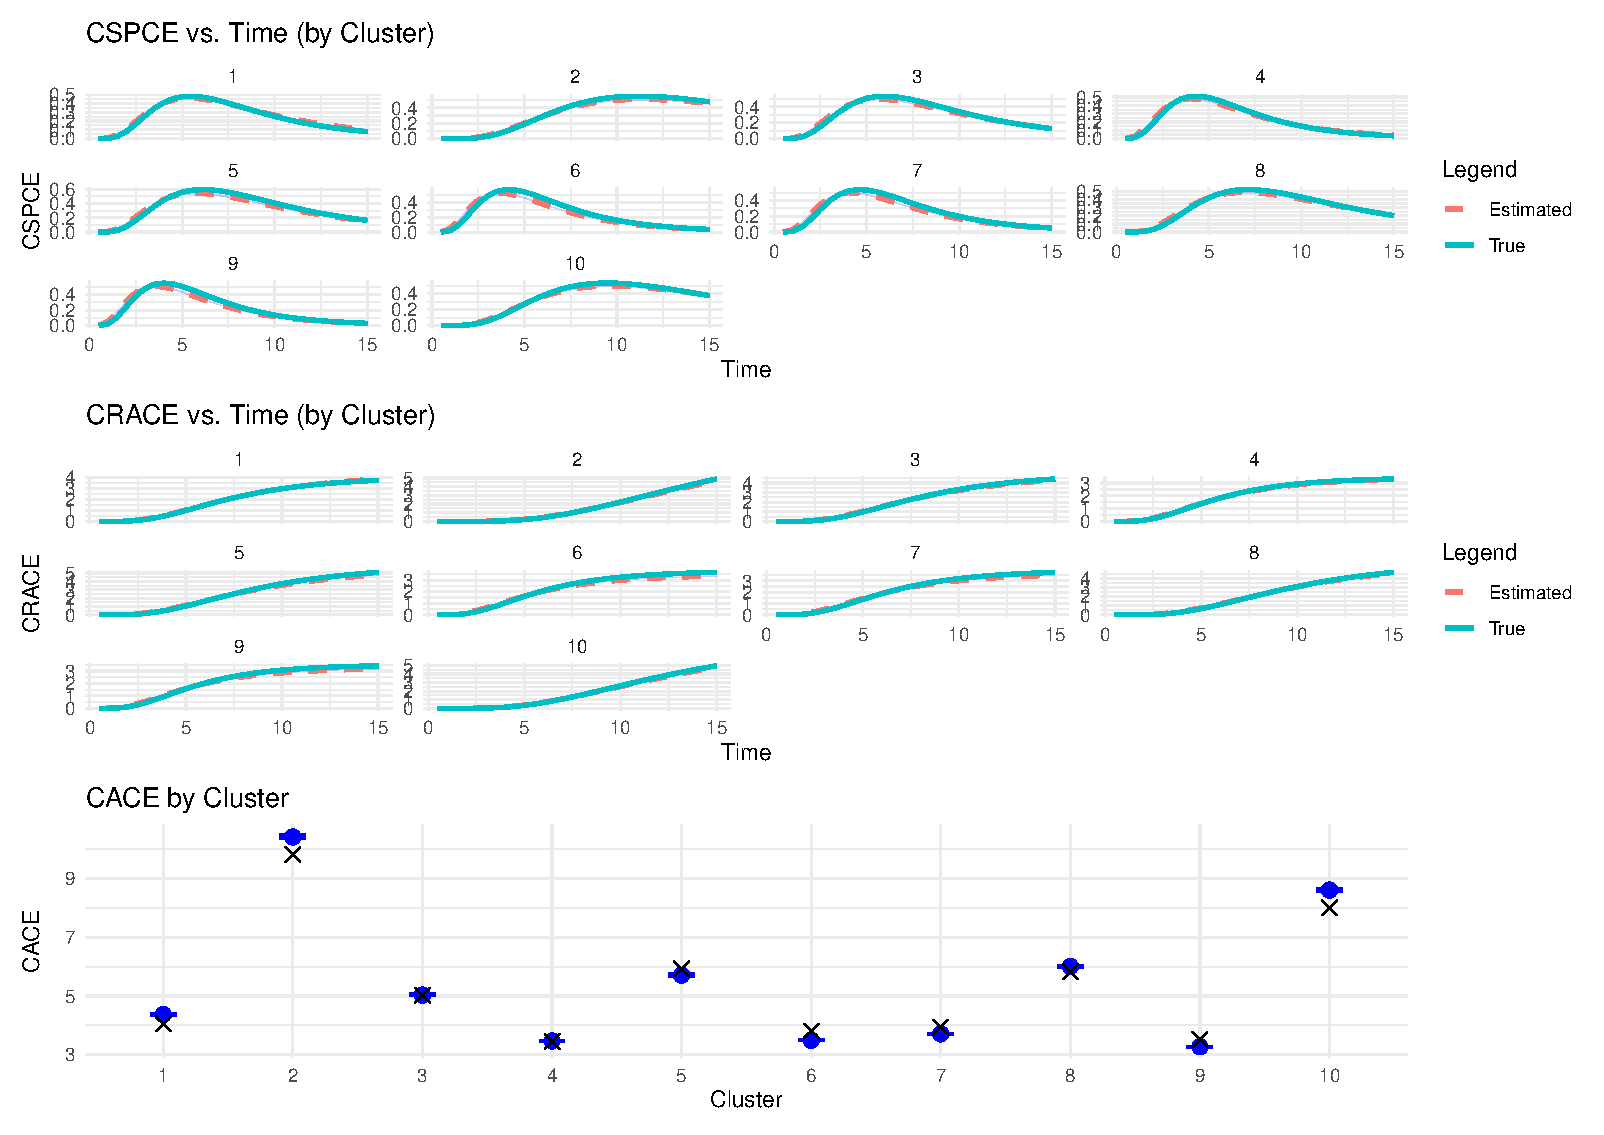
\includegraphics[height=.8\linewidth]{pics/Sim4.pdf}
\end{frame}

\begin{frame}{Results (Rep1)}
  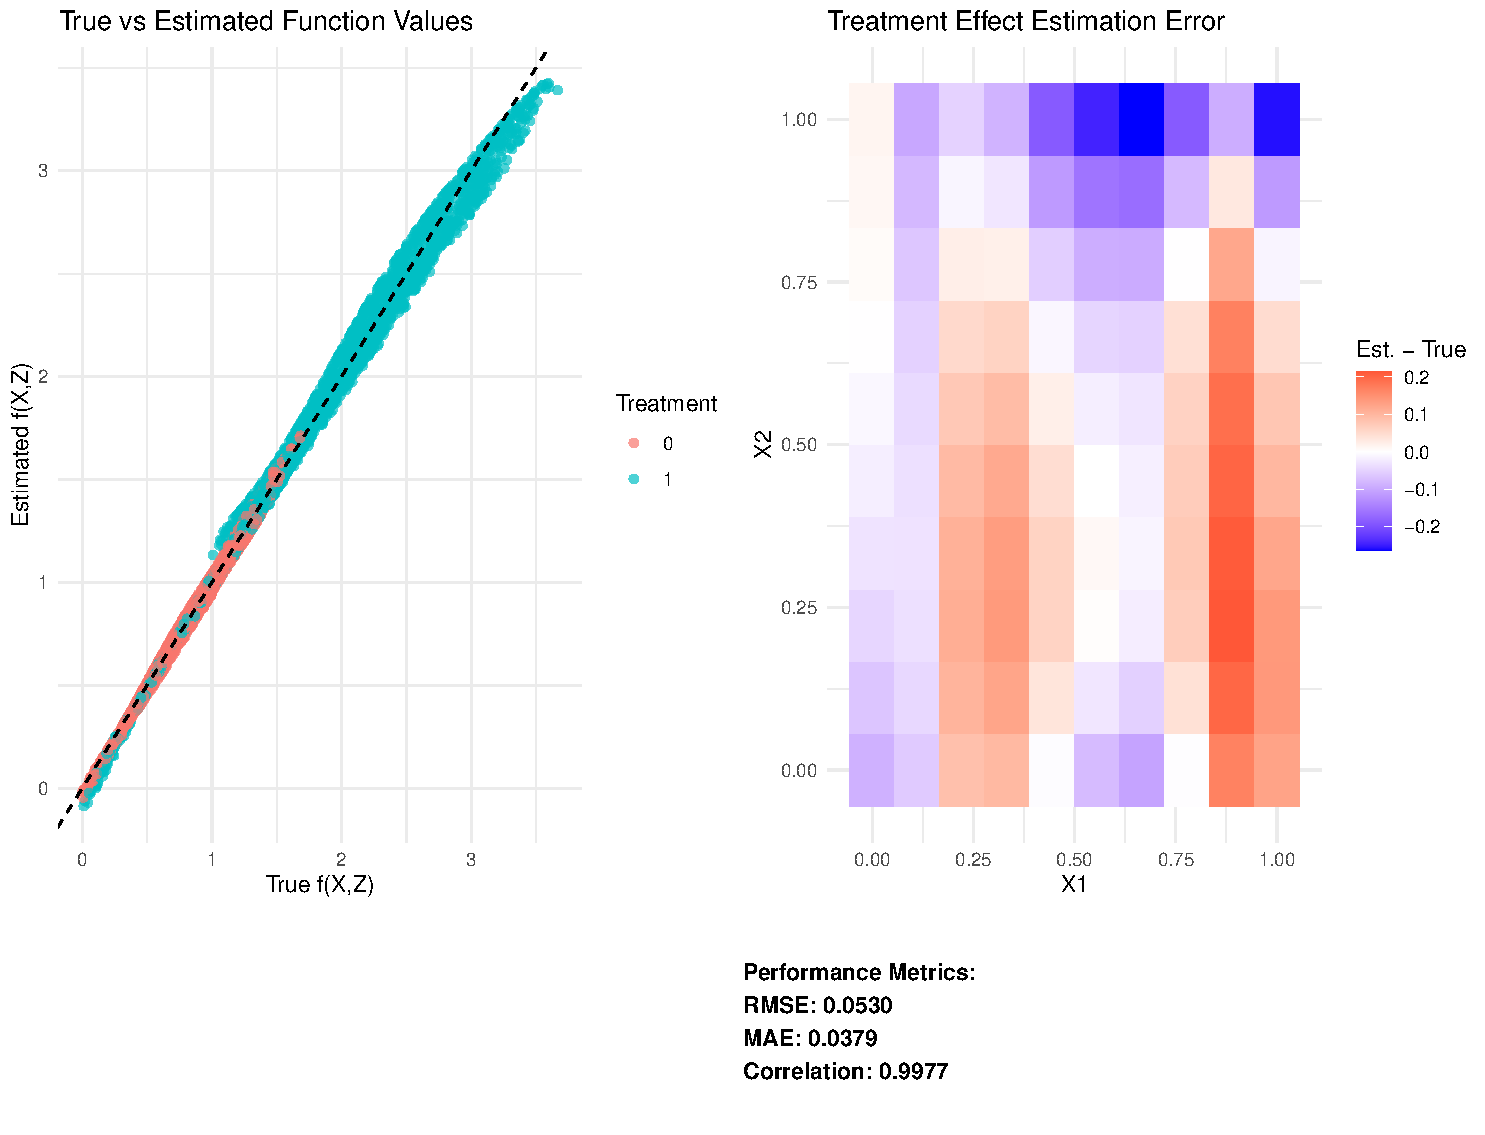
\includegraphics[height=.8\linewidth]{pics/Sim4_2.pdf}
\end{frame}

\begin{frame}{Results (Rep2)}
    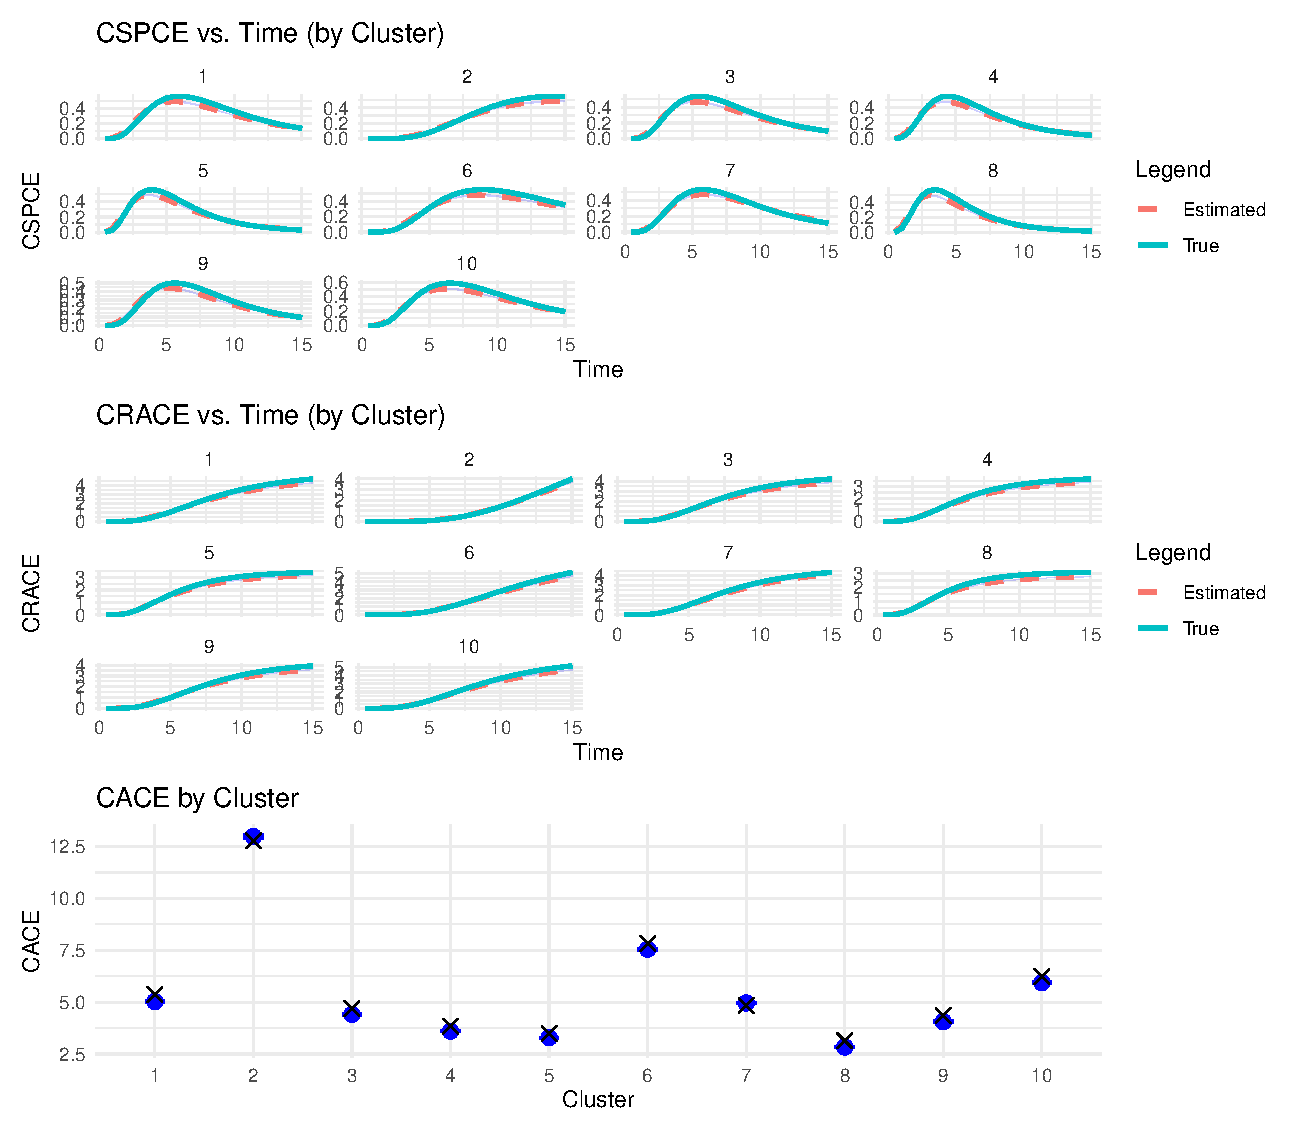
\includegraphics[height=.8\linewidth]{pics/Sim4_rep2.pdf}
\end{frame}

\begin{frame}{Results (Rep2)}
  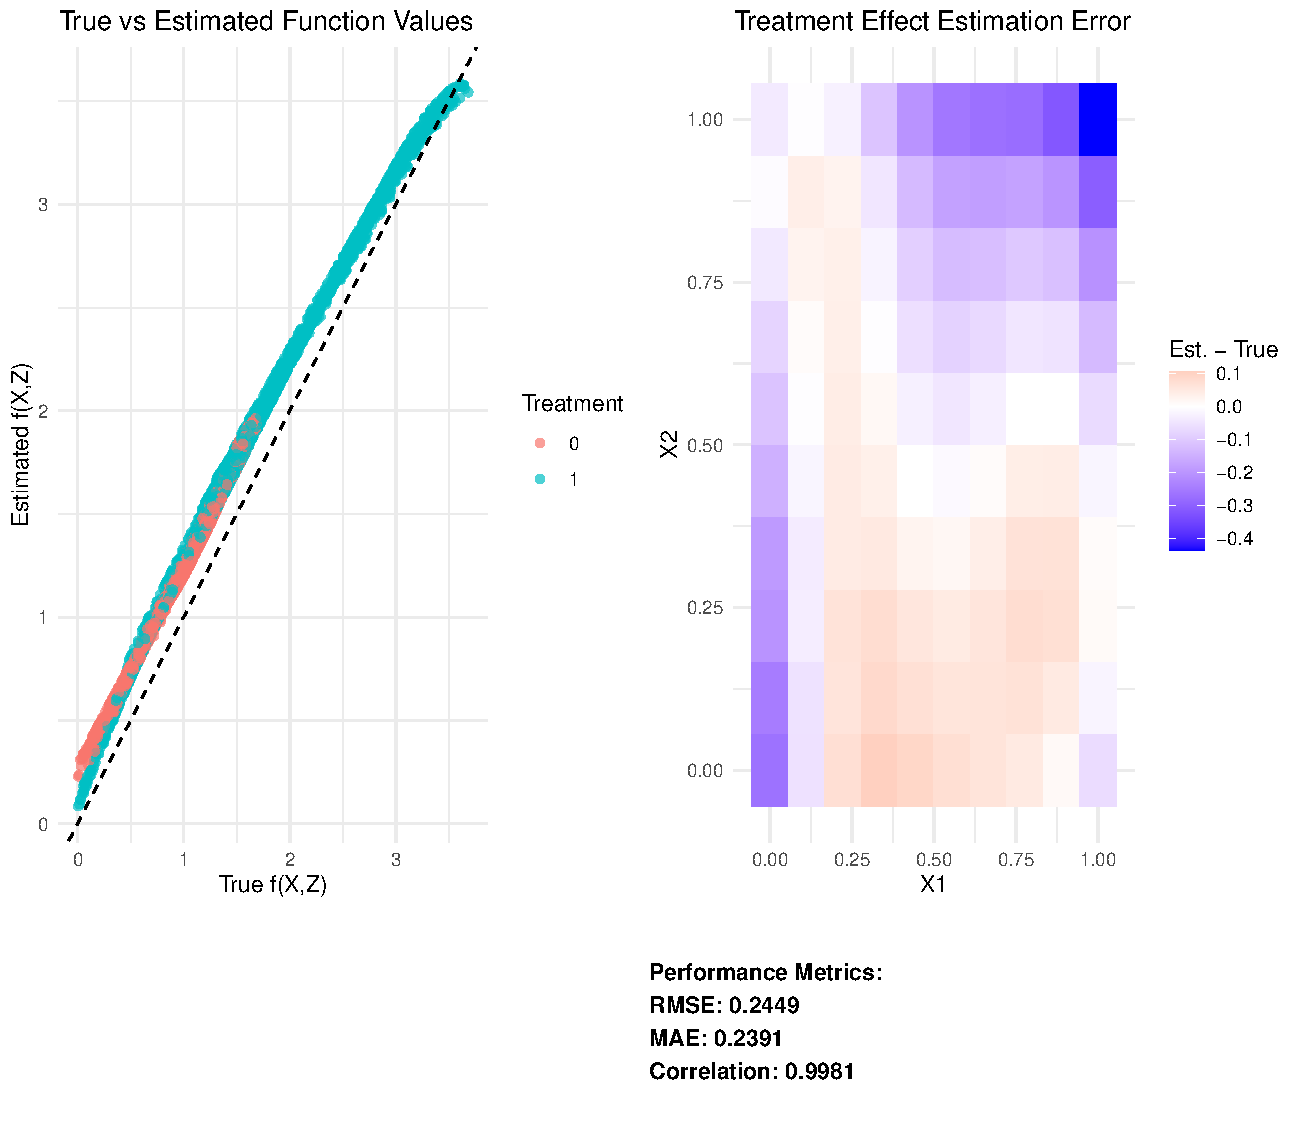
\includegraphics[height=.8\linewidth]{pics/Sim4_rep2_2.pdf}
\end{frame}

\begin{frame}{Results (Rep3)}
  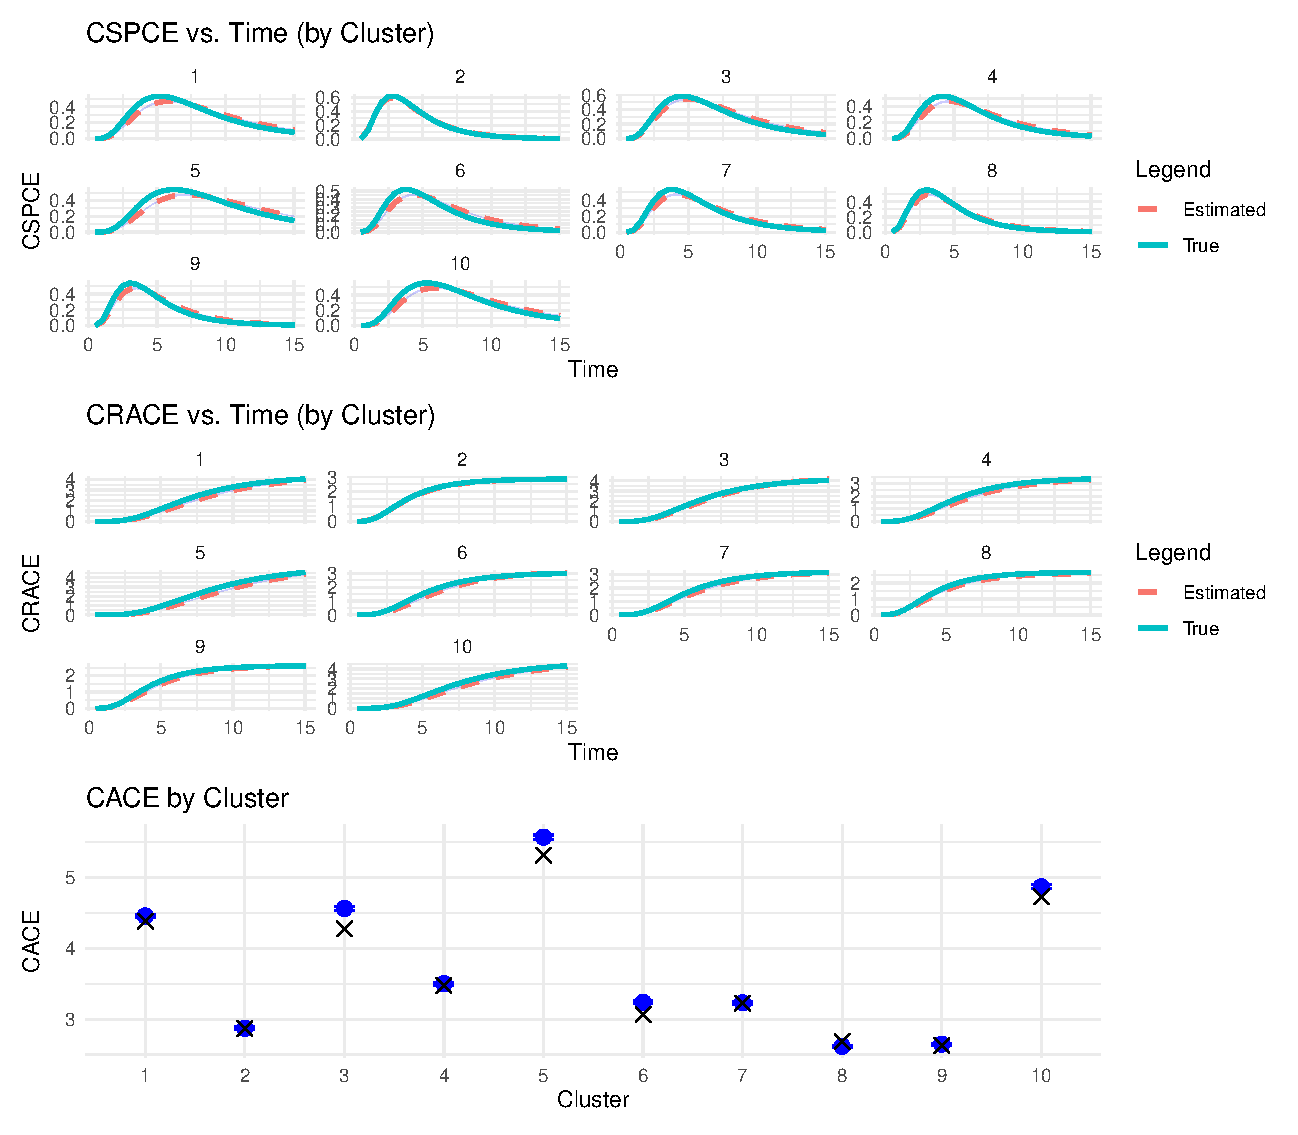
\includegraphics[height=.8\linewidth]{pics/Sim4_rep3.pdf}
\end{frame}

\begin{frame}{Results (Rep3)}
  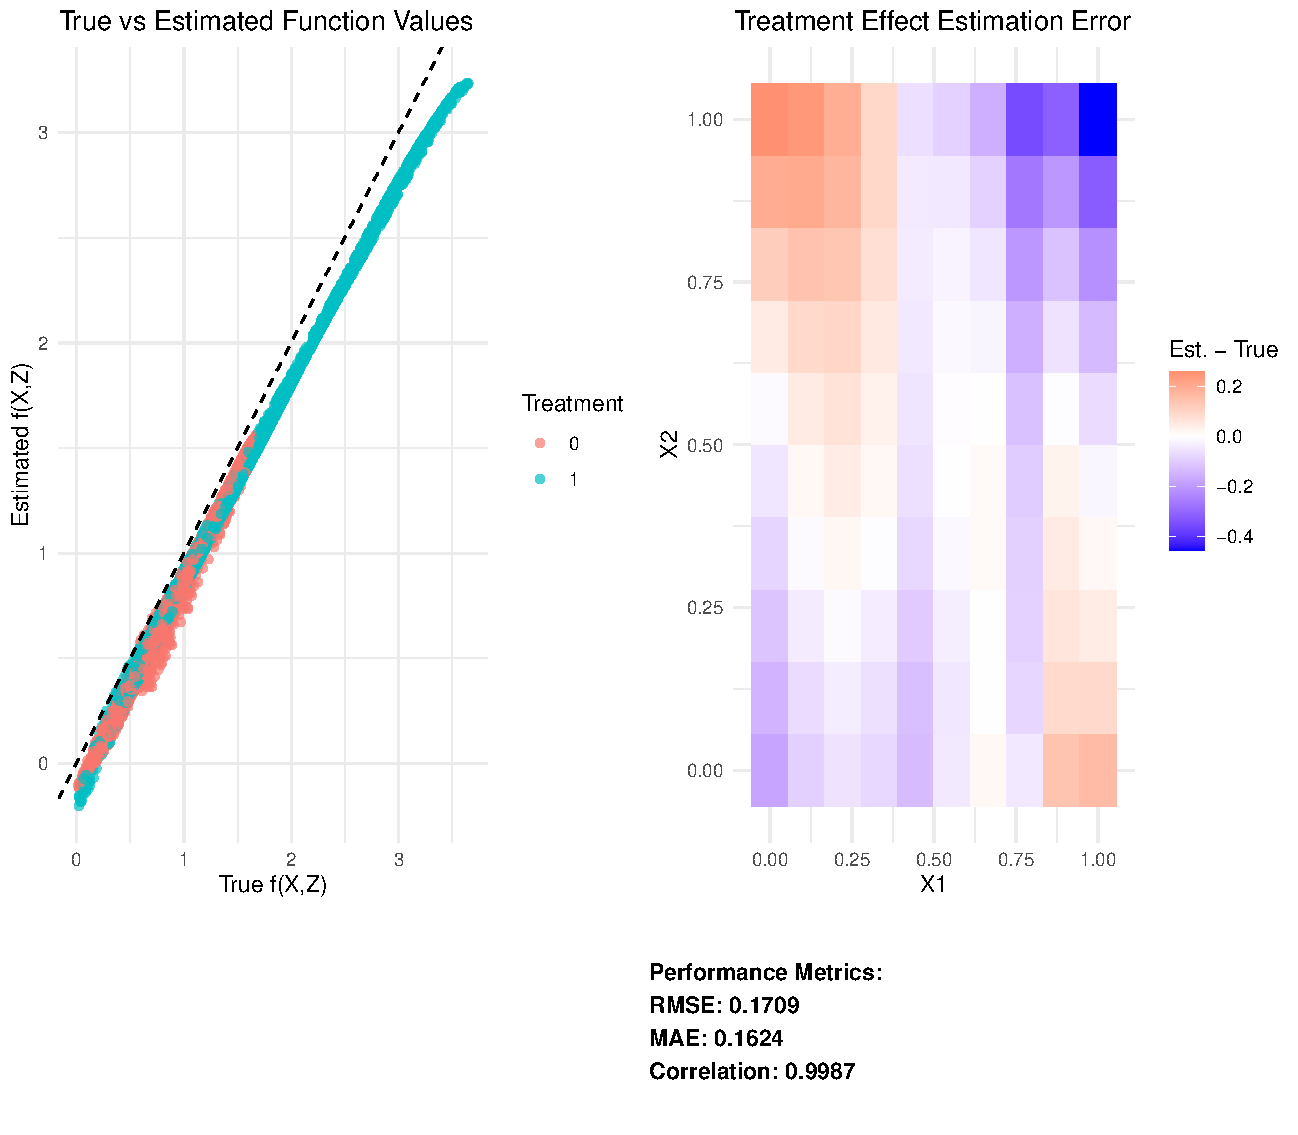
\includegraphics[height=.8\linewidth]{pics/Sim4_rep3_2.pdf}
\end{frame}

\begin{frame}{}
  \vspace{40pt}
  \centering
  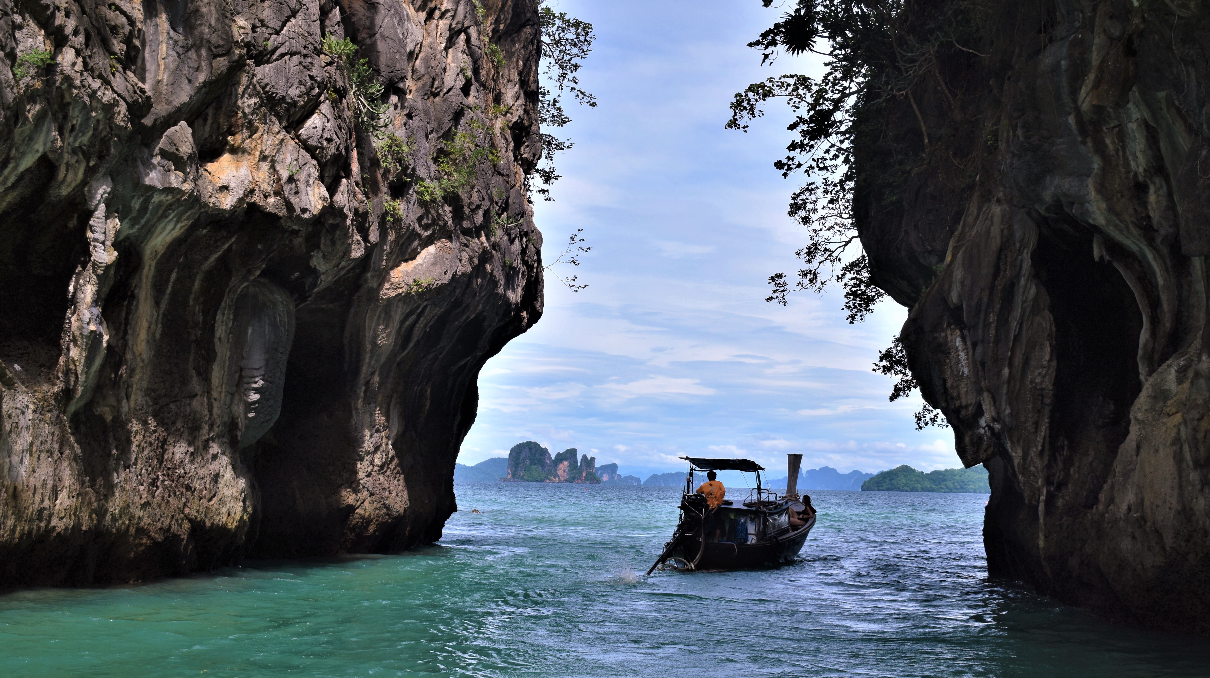
\includegraphics{pics/thankyou.png}
  \Huge{\textbf{Thank you!}}
  \vspace{40pt}
\end{frame}

\end{document}